\documentclass[pdftex,12pt,a4paper]{article}

\usepackage[pdftex]{graphicx}
\usepackage{paralist}
\usepackage{mathtools}
\usepackage{hyperref}
\usepackage[xindy]{glossaries}

\newcommand{\HRule}{\rule{\linewidth}{0.5mm}}

\newglossaryentry{OpenGL}
{
  name=OpenGL,
  description={stands for Open Graphics Library and is a cross-language, multi-platform application programming interface (API) for rendering 2D and 3D computer graphics\footnote{http://en.wikipedia.org/wiki/OpenGL}}
}

\newglossaryentry{OpenGL ES}
{
  name=OpenGL ES,
  description={OpenGL for Embedded Systems (OpenGL ES) is a subset of the OpenGL computer graphics rendering application programming interface (API) for rendering 2D and 3D computer graphics such as those used by video games, typically hardware-accelerated using a graphics processing unit (GPU)\footnote{http://en.wikipedia.org/wiki/OpenGL\_ES}}
}

\newglossaryentry{Versor (libvsr)}
{
  name=Versor (libvsr),
  description={is a C++ Library for Geometric Algebra with built-in draw routines\footnote{https://github.com/wolftype/vsr2.0/}}
}

\newglossaryentry{geometric algebra}
{
  name=Geometric Algebra (GA),
  description={is the Clifford algebra of a vector space over the field of real numbers endowed with a quadratic form \footnote{http://en.wikipedia.org/wiki/Geometric\_algebra}}
}

\newglossaryentry{GLV}
{
  name=GLV,
  description={is a GUI building toolkit written in C++ for Linux, OSX, and Win32\footnote{https://github.com/AlloSphere-Research-Group/GLV}}
}

\newglossaryentry{GFX}
{
  name=GFX,
  description={is a generic graphics library (using OpenGL and OpenGL ES 2.0)\footnote{https://github.com/wolftype/gfx}}
}

\newglossaryentry{bivector}
{
  name=Bivector,
  description={is a quantity in exterior algebra or geometric algebra that extends the idea of scalars and vectors\footnote{http://en.wikipedia.org/wiki/Bivector}}
}

\newglossaryentry{GLUT}
{
  name=GLUT,
  description={stands for OpenGL Utility Toolkit and is a library of utilities for OpenGL programs, which primarily perform system-level I/O with the host operating system\footnote{http://en.wikipedia.org/wiki/OpenGL\_Utility\_Toolkit}}
}

\newglossaryentry{cube mapping}
{
  name=Cube mapping,
  description={is a method of environment mapping that uses the six faces of a cube as the map shape within the field of computer graphics\footnote{http://en.wikipedia.org/wiki/Cube\_mapping}}
}
\makeglossaries


\begin{document}
%deckblatt start
\thispagestyle{empty}
\begin{center}
\Large{Berne University of Applied Sciences (BFH)}\\
\end{center}
 
 
\begin{center}
\Large{Department Engineering and information technology}
\end{center}
\begin{verbatim}
\end{verbatim}
\begin{center}
\textbf{\LARGE{BZG1310 -  Object-oriented geometry}}
\end{center}
\begin{verbatim}
 
 
\end{verbatim}
\begin{center}
\textbf{Documentation Project 1}
\end{center}
\begin{verbatim} 
\end{verbatim}
 
\begin{flushleft}
\begin{tabular}{lll}
\textbf{Subject:} & & Spinning cube with spheres on its edges --\\
& & Classical approach using OpenGL and GLSL\\
& & \\
& & \\
& & \\
\textbf{Student:} & & Sven Osterwalder (ostes2@bfh.ch)\\
& & \\
& & \\
\textbf{Date:} & & {\today}\\
& & \\
& & \\
\textbf{Professor:} & & M. Stampfli
\end{tabular}
\end{flushleft}

\newpage

\section{Management summary}

This dissertation is part of a project in the context of the subject \textit{BZG1310: Object-oriented geometry} at Bern University of Applied Sciences.
\\
\\
One goal of this project is the implementation of a rotating cube which has a sphere on each edge using classical approaches within the field of computer graphics (e.g. matrices or quaternions).
\\
\\
The goal could be reached and the task was implemented using C++, \gls{OpenGL} and \gls{GLSL} and matrices.\\
\\
\begin{figure}[htbp]
\centering \rotatebox{0}{\scalebox{0.2}[0.2]{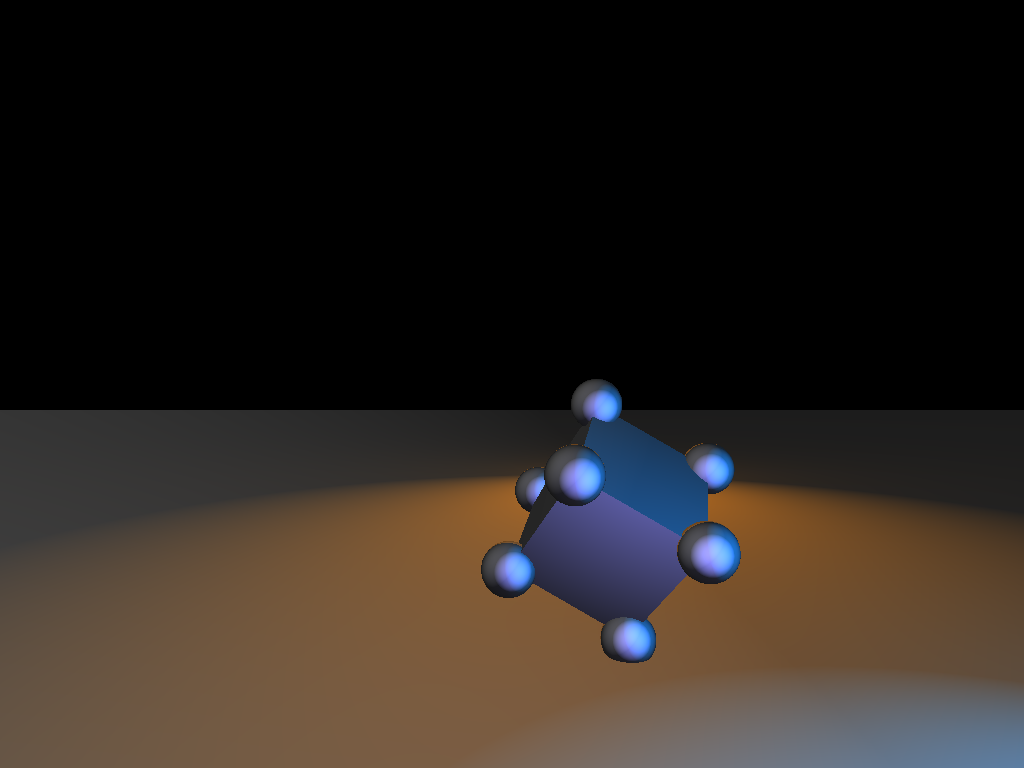
\includegraphics{screenshot.png}}}
\caption{Screenshot of the running application \label{fig:screenshot}}
\end{figure}

\section{Implementation}

The implementation was done using C++, OpenGL and the shader language GLSL.

\subsection{Framework}

To cover the main tasks such as providing minimal application logic, loading files (models, textures and shaders) or handling input, a minimal framework based upon \gls{GLEW}, \gls{ASSIMP} and \gls{GLFW} was built.\\
\newpage
The framework consists the following aspects:
\begin{compactitem}
	\item Main routine (initializing, running and finishing the application)
	\item Camera handling
	\item Helper class for mathematical functions (consisting vectors and matrices)
	\item Representation of light through shaders based on GLSL
	\item Model loading using ASSIMP library
	\item A pipeline for performing transformations
	\item Management of textures using \gls{ImageMagick}
	\item Common utilities (e.g. for loading files into memory)
\end{compactitem}

\subsection{Main process}

In general the following is done when executing the application:
\begin{compactitem}
	\item Initialization of the application
	\item Execution of the application until a quit event is received
	\item Termination of the application
\end{compactitem}

\subsection{Geometric operations}

As the geometric operations are the main aspect of the course BZG1310, this section shows how this aspect was realized within the application.\\
To perform the needed translations, rotations and scaling of the objects, matrix multiplication was used.\\
\\
As basis for the representation, perspective projection was used in form of matrices, which represent the world space, as well as a camera.\\
\\
The positions as well as the rotations are represented resp. implemented using three dimensional vectors, the scaling is implemented using four dimensional matrices.\\
\\
The procedure for calculating the positions and the rotation of objects is as follows:
\begin{compactitem}
	\item Setting the world position according to the current object:\\
		\noindent\hspace*{10mm} $ worldTranslationtionMatrix := $\\
			\\
			\noindent\hspace*{15mm} $
			\begin{bmatrix}
			1.0 & 0.0 & 0.0 & object.X \\
			0.0 & 1.0 & 0.0 & object.Y \\
			0.0 & 0.0 & 1.0 & object.Z \\
			0.0 & 0.0 & 0.0 & 1.0
			\end{bmatrix}
			$ \\
			\\
	\item Setting the world rotation according to the current object:\\
		\noindent\hspace*{10mm} $ worldRotationMatrix := rotationZ * rotationY * rotationX $\\
		\\
		\noindent\hspace*{10mm} $ rotationX := $\\
				\\
				\noindent\hspace*{15mm} $
				\begin{bmatrix}
				1.0 & 0.0 & 0.0 & 0.0 \\
				0.0 & cos(object.X) & -sin(object.X) & 0.0 \\
				0.0 & sin(object.X) & cos(object.X) & 0.0 \\
				0.0 & 0.0 & 0.0 & 1.0
				\end{bmatrix}
				$ \\
				\\
		\noindent\hspace*{10mm} $ rotationY := $\\
				\\
				\noindent\hspace*{15mm} $
				\begin{bmatrix}
				cos(object.Y) & 0.0 & -sin(object.Y) & 0.0 \\
				0.0 & 1.0 & 0.0 & 0.0 \\
				sin(object.Y) & 0.0 & cos(object.Y) & 0.0 \\
				0.0 & 0.0 & 0.0 & 1.0
				\end{bmatrix}
				$ \\
				\\
		\noindent\hspace*{10mm} $ rotationZ := $\\
				\\
				\noindent\hspace*{15mm} $
				\begin{bmatrix}
				cos(object.Z) & -sin(object.Z) & 0.0 & 0.0 \\
				sin(object.Z) & cos(object.Z) & 0.0 & 0.0 \\
				0.0 & 0.0 & 1.0 & 0.0 \\
				0.0 & 0.0 & 0.0 & 1.0
				\end{bmatrix}
				$ \\
				\\
	\item Getting the world transformation:\\
		\noindent\hspace*{10mm} $ worldTransformation := worldTranslationMatrix * worldRotationMatrix $\\
	\item Set the world matrix:\\
		\noindent\hspace*{10mm} $ worldMatrix := worldTransformation * scalingOfTheCurrentObject $\\
	\item Repeat the steps above for the world perspective
\end{compactitem}
\vspace*{2mm}
\noindent\hspace*{0mm}As one can see, with the routine above the objects get first rotated (locally) and then translated to a specific point in space which concerns only the cube. Additionally the same procedure gets done for objects rotating around a so called pivot - a relative point in space. This is needed to keep the spheres performing the same rotation as the cube in addition to their own local rotation.\\
\newpage
\noindent The only difference is hereby that the world transformation needs to be done respecting the provided point in form of a four dimensional matrix and by changing the order of the multiplication, which results in the following:\\
\\
\noindent\hspace*{10mm} $ worldTransformation := \\
	\noindent\hspace*{17mm} providedPointMatrix *\\
	\noindent\hspace*{17mm} worldRotationMatrix *\\
	\noindent\hspace*{17mm} worldTranslationMatrix $

\section{Conclusion}
The project was a bit effortful but also great fun to do. I could sure have chosen a less effortful way to realize the project but I chose this way as the subject area is one of my main interests and I was concerning myself before with this topic. It especially helped me to get a deeper understanding about how to implement the theory into a practical application.

\printglossary[numberedsection]

\end{document}